\chapter{Statistics and Experiments}

% =============================================================================
\section{Statistics}

\subsection{\texttt{STAT\_001} - Group Courses by Credits}

This experiment plots the number of courses for each possible number of credits
in a bars chart. The results of this was listed in
table~\ref{tab:courses_credits}.

\subsection{\texttt{STAT\_002} - List Domain of Courses Fields}

Gets domain of the fields of courses. Relevant results are listed in some
tables in section~\ref{sec:data_courses}.

\subsection{\texttt{STAT\_003} - Number of Courses per Degree}

A list of courses per degree is computed. This gives an idea of how many
courses there are in a given degree. A list of courses per degree and semester
is also given to give an idea of how the courses are distributed across the two
semesters.

Tables~\ref{tab:stat_003_res_1} and~\ref{tab:stat_003_res_2} show these results.

It should be noticeable that some degrees only have courses in one semester.
The names of the degrees are not available, only their codes. But it is
noticeable that the degree with the greater number of courses is
\texttt{B\_M\_REST\_EINF\_E}, which appears to be an Informatics Master's
Degree.

\begin{table}[h!]
    \centering

    \begin{tabular}{l r}
        Degree                             & CourseCodeMoodle \\ \hline
        \texttt{B\_M\_EHEA (478)}          & 7                \\
        \texttt{B\_M\_REST\_EINF\_E (578)} & 28               \\
        \texttt{B\_M\_REST\_TET (457)}     & 7                \\
        \texttt{B\_PD\_M\_E (580)}         & 8                \\
        \texttt{CCDND\_CPM (344)}          & 1                \\
        \texttt{FC\_CVP\_FDOC (513)}       & 2                \\
        \texttt{FC\_CVP\_UAM (514)}        & 3                \\
        \texttt{FC\_EDM (564)}             & 1                \\
        \texttt{PG\_B\_AE (438)}           & 10               \\
        \texttt{PG\_B\_EGNEG (554)}        & 10               \\
    \end{tabular}

    \caption
        [Number of Courses per Degree]
        {Number of Courses per Degree.}

    \label{tab:stat_003_res_1}
\end{table}

\begin{table}[h!]
    \centering

    \begin{tabular}{l l r}
        Degree                             & Semester       & CourseCodeMoodle \\ \hline
        \texttt{B\_M\_EHEA (478)}          & \textit{Par}   & 3                \\
                                           & \textit{Ímpar} & 4                \\
        \texttt{B\_M\_REST\_EINF\_E (578)} & \textit{Par}   & 14               \\
                                           & \textit{Ímpar} & 14               \\
        \texttt{B\_M\_REST\_TET (457)}     & \textit{Par}   & 2                \\
                                           & \textit{Ímpar} & 5                \\
        \texttt{B\_PD\_M\_E (580)}         & \textit{Par}   & 3                \\
                                           & \textit{Ímpar} & 5                \\
        \texttt{PG\_B\_EGNEG (554)}        & \textit{Par}   & 4                \\
                                           & \textit{Ímpar} & 5                \\
        \texttt{PG\_B\_AE (438)}           & \textit{Par}   & 5                \\
                                           & \textit{Ímpar} & 5                \\
        \texttt{FC\_EDM (564)}             & \textit{Par}   & 1                \\
        \texttt{CCDND\_CPM (344)}          & \textit{Ímpar} & 1                \\
        \texttt{FC\_CVP\_FDOC (513)}       & \textit{Ímpar} & 2                \\
        \texttt{FC\_CVP\_UAM (514)}        & \textit{Ímpar} & 3                \\
    \end{tabular}

    \caption
        [Number of Courses per Degree and Semester]
        {Number of Courses per Degree and Semester.}

    \label{tab:stat_003_res_2}
\end{table}

\subsection{\texttt{STAT\_004} - Plotting Activity of Students over the
Semester}

To look for patterns in the usage of Moodle we look into plotting the activity
of students over the courses over a semester. The six courses with the greatest
number of activities are chosen and for each of them two plots are made.

One plot displays the overall number of~\gls{crud} activities over the semester
and the number of \textbf{C}reate activities, \textbf{R}ead activities, etc.
Figure~\ref{fig:stat_004_all} show these plots for two courses. As it can be
seen, the number of Read activities is far greater then the others, which is to
be expected since to do any other activity, at least a Read activity has to
take place. For example, a student needs to open the Moodle page, and therefore
do a Read, to deliver a project, and therefore do a Create.

It is hypothesis that the number is also greater because students will usually
just read new messages in the Moodle, or consult new materials, without doing
any other activity.

The second plot made to each course is similar, but only the Create, Update,
and Delete activities are plotted. Figure~\ref{fig:stat_004_cud} show two
examples these plots. Notice that the number of creates is not always greater
then the number of updates, and vice-versa. But the number of deletes is always
below creates and updates. This concludes that the delete activity is simply
not that common.

\begin{figure}[h!]
    \centering

    \begin{subfigure}{.5\textwidth}
        \centering
        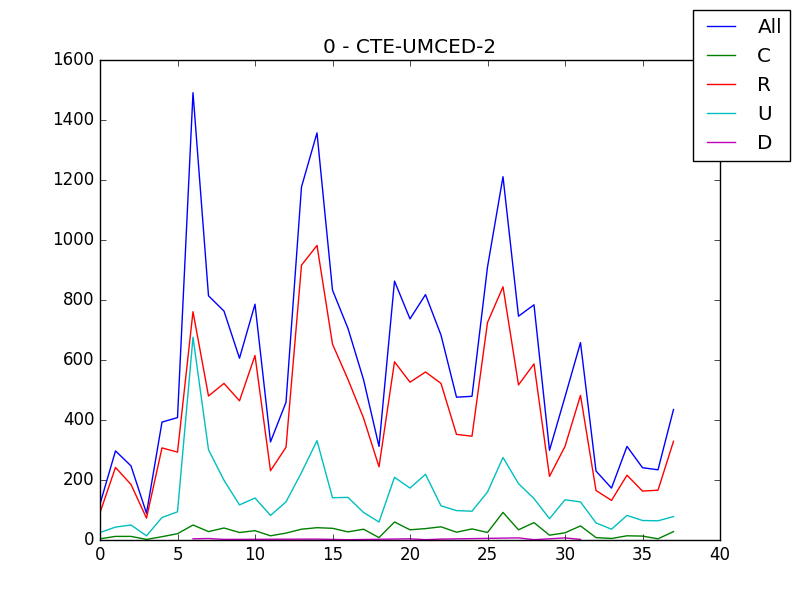
\includegraphics[width=\linewidth]{../src/stat_004_results/fig_0_CTE-UMCED-2_all}
        \label{subfig:stat_004_0_all}
    \end{subfigure}%
    \begin{subfigure}{.5\textwidth}
        \centering
        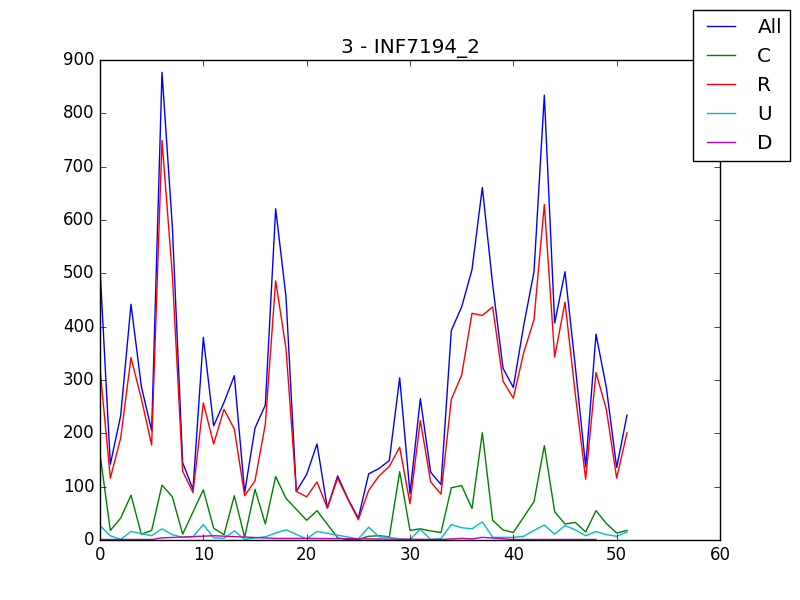
\includegraphics[width=\linewidth]{../src/stat_004_results/fig_3_INF7194_2_all}
        \label{subfig:stat_004_3_all}
    \end{subfigure}

    \caption
        [Stat 004 plots for all activities]
        {Stat 004 plots for all activities.}

    \label{fig:stat_004_all}
\end{figure}

\begin{figure}[h!]
    \centering

    \begin{subfigure}{.5\textwidth}
        \centering
        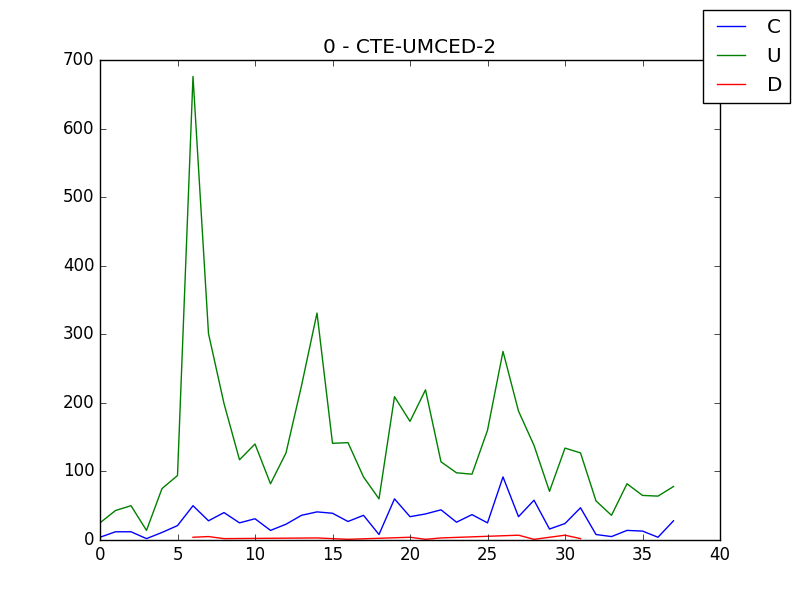
\includegraphics[width=\linewidth]{../src/stat_004_results/fig_0_CTE-UMCED-2_cud}
        \label{subfig:stat_004_0_cud}
    \end{subfigure}%
    \begin{subfigure}{.5\textwidth}
        \centering
        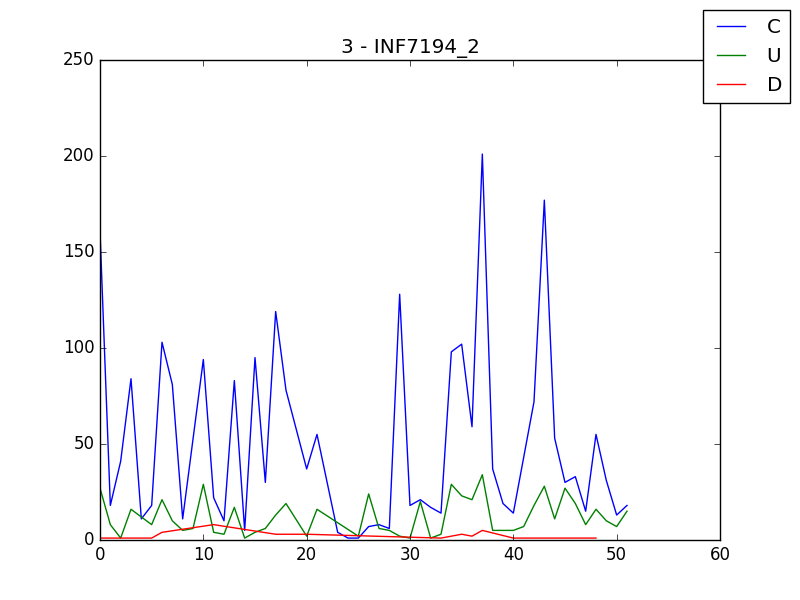
\includegraphics[width=\linewidth]{../src/stat_004_results/fig_3_INF7194_2_cud}
        \label{subfig:stat_004_3_cud}
    \end{subfigure}

    \caption
        [Stat 004 plots for C, U, and D activities]
        {Stat 004 plots for C, U, and D activities.}

    \label{fig:stat_004_cud}
\end{figure}

\subsection{\texttt{STAT\_005} - Total Number of Activities vs Mean of
Activities per Week}

This analysis attempts to understand if the activities of courses remain the
same as the semester goes on. So the mean of the activities per course and week
is plotted, as it is displayed in figure~\ref{fig:stat_005}. The total number
of activities is also plotted in figure~\ref{fig:stat_005}.

It is visible that, although the number of activities drops as the semester
goes on, the mean number of activities stayed relatively the same despite
varying a lot. This is due to the fact that some courses stop being active as
the semester goes on, as it will be shown in section~\ref{sec:stat_006}, but
despite that, the courses that do remain active don't register a drop of
activity as time goes on.

\begin{figure}[h!]
    \centering

    \includegraphics[width=\linewidth]{../src/stat_005_results/plot}

    \caption
        [Total Number of Activities vs Mean of Activities per Week]
        {Total Number of Activities vs Mean of Activities per Week.}

    \label{fig:stat_005}
\end{figure}

\subsection{\texttt{STAT\_006} - Number of Active Courses vs Number of
Activities}
\label{sec:stat_006}

A correlation is found between the total number of activities and the number of
active courses per week. The total number of active courses in a week is
plotted as a bars chart in figure~\ref{fig:stat_006}, along with the total
number of activities.

An course ceases to be active on a given week where it no longer has activities
after that week. For example, suppose a course has activities on weeks, 0, 1,
4, and 8. Then the course is only active until week 8.

The number of activities goes down with the number of active courses, as it
would be expected. But around weeks 30 to 50, it is visible that the number of
activities significantly drops from the number of courses, as opposed to the
first weeks where the numbers are much more similar. This is +probably due to
students incising lack of interest in courses' activities as the semester goes
on, which is normal behaviour.

\begin{figure}[h!]
    \centering

    \includegraphics[width=\linewidth]{../src/stat_006_results/plot}

    \caption
        [Active Courses vs Number of Activities]
        {Active Courses vs Number of Activities.}

    \label{fig:stat_006}
\end{figure}

% =============================================================================
\section{Experiments}
